\chapter{Results}
\begin{center}
\vspace{-6ex}
\textit{"Cut to the chase"}
\vspace{6ex}
\end{center}

\section{Data set 1}

\subsection{Image segmentation}

\begin{figure}[]
    \centering
    \captionsetup[subfigure]{justification=centering}
    \begin{subfigure}[b]{0.3\textwidth}
        \centering
        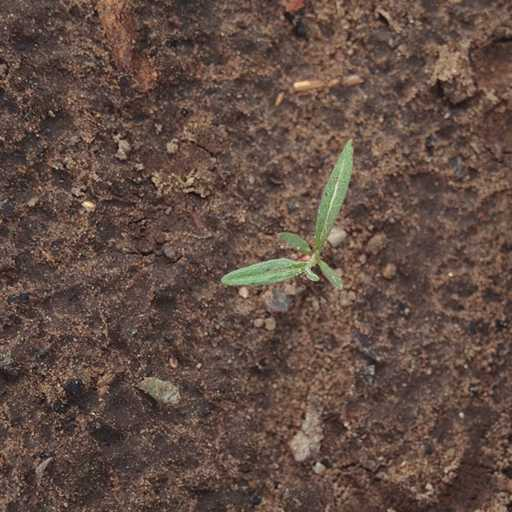
\includegraphics[width=\textwidth]{./figure/result/segmentation/imgORIGINAL.png}
		\caption{}
		\label{fig:seg_a}
    \end{subfigure}
    \begin{subfigure}[b]{0.3\textwidth}
        \centering
        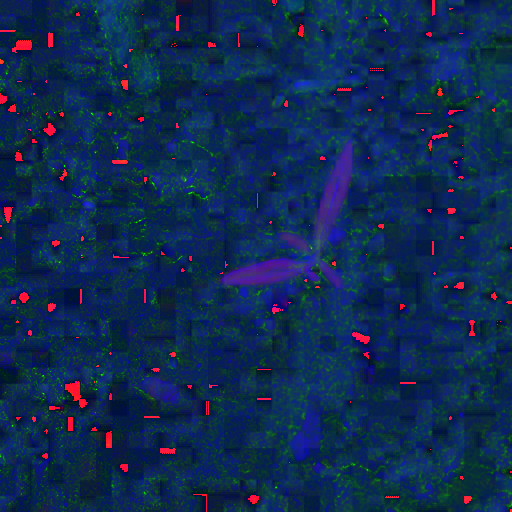
\includegraphics[width=\textwidth]{./figure/result/segmentation/imgHSI.png}
        \caption{}
		\label{fig:seg_b}
    \end{subfigure}
    \begin{subfigure}[b]{0.3\textwidth}
        \centering
        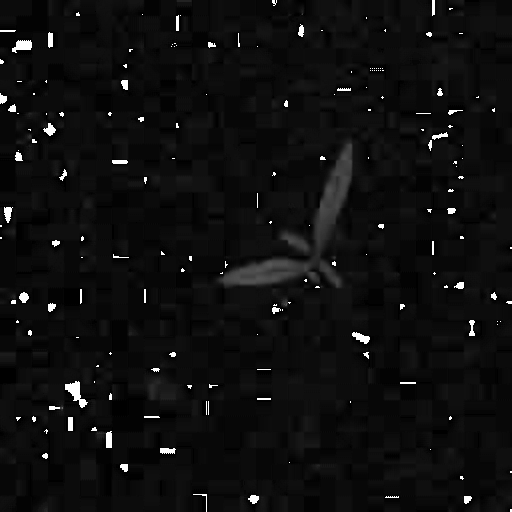
\includegraphics[width=\textwidth]{./figure/result/segmentation/imgHSI1.png}
		\caption{}
		\label{fig:seg_c}
    \end{subfigure}
    \begin{subfigure}[b]{0.3\textwidth}
        \centering
        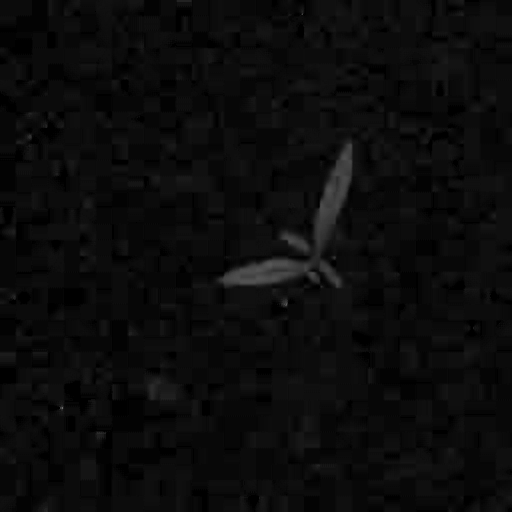
\includegraphics[width=\textwidth]{./figure/result/segmentation/imgHSIClean.png}
		\caption{}
		\label{fig:seg_d}
    \end{subfigure}
    \begin{subfigure}[b]{0.3\textwidth}
        \centering
        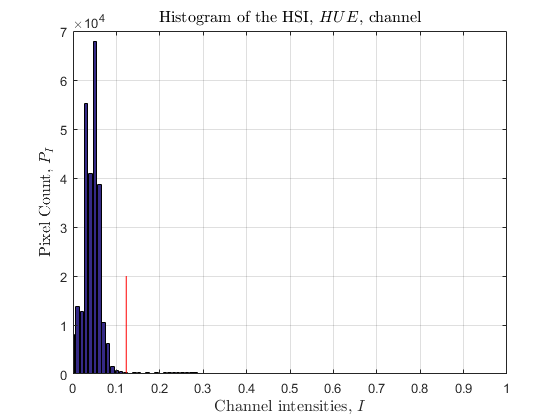
\includegraphics[width=\textwidth]{./figure/result/segmentation/imgCLIPPING.png}
		\caption{}
		\label{fig:seg_e}
    \end{subfigure}
    \begin{subfigure}[b]{0.3\textwidth}
        \centering
        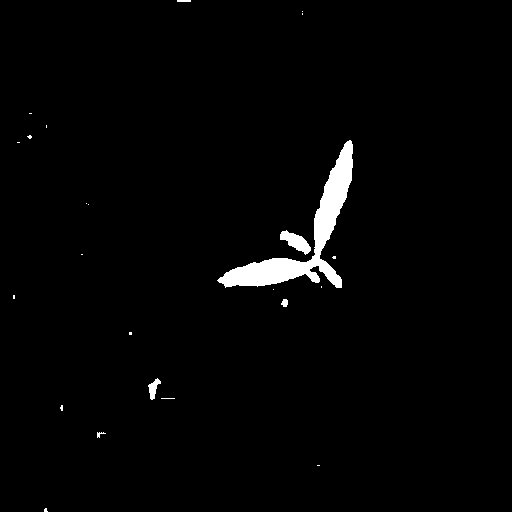
\includegraphics[width=\textwidth]{./figure/result/segmentation/imgHSIThreshold.png}
		\caption{}
		\label{fig:seg_f}
    \end{subfigure}
    \begin{subfigure}[b]{0.3\textwidth}
        \centering
        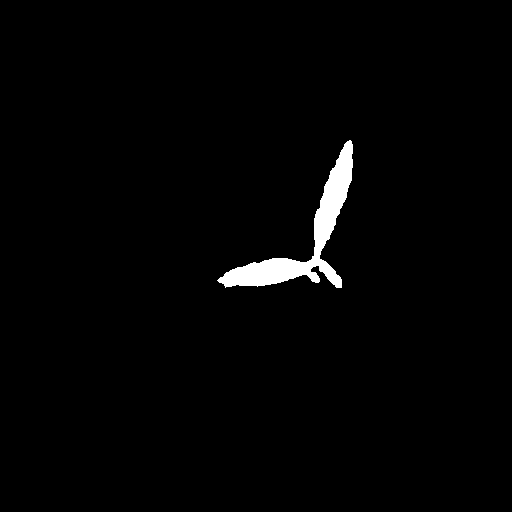
\includegraphics[width=\textwidth]{./figure/result/segmentation/imgHSIThresholdClean.png}
		\caption{}
		\label{fig:seg_g}
    \end{subfigure}
    \begin{subfigure}[b]{0.3\textwidth}
        \centering
        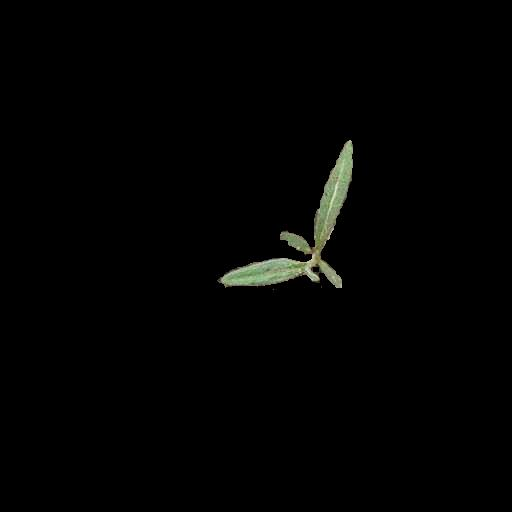
\includegraphics[width=\textwidth]{./figure/result/segmentation/imgSEG.png}
		\caption{}
		\label{fig:seg_h}
    \end{subfigure}
    \caption{The segmentation process as follows: \textit{(a):} The original image is loaded and prepared for processing. \textit{(b):} The image converted to HSI but still represented in RGB colours by the computer. \textit{(c):} For the segmentation to work properly the image needs to be represented in one channel that represents the two segments well, and this is what the Hue channel in HSI representation does. \textit{(d):} The Hue channel clean up. \textit{(e):} The optimal threshold, using the global adaptive thresholding, between the two segments is represented by the red line  \textit{(f):} Binarization of the HSI image using segmentation. \textit{(g):} Clean up the binary image by removing small objects using the connected component sizes as measure. \textit{(h):} Final segmented image.  }
    \label{fig:1}
\end{figure}

The first thing we are doing on the data set is to extract the objects we want to use for the later stages of the classification process. During this stage we want to segment the images to only keep the plants that are to be classified in that image. In Chapter.~\ref{chap:imgPro} we discussed the different parts necessary for this process. This data set, as we can see in Figure.~\ref{fig:seg_f}, uses different colors for the relevant object in contrast to the background, namely greenish versus brownish. The image is thus segmented using the Hue value of the pixels. We can see from the result of the segmentation in Figure.~\ref{fig:seg_h} that the most part of the plant is a part of the object and a small portion of the background is remaining. This provides a solid foundation for the machine learning algorithms as we have a only a small amount of noise in the resulting object.

\subsection{Plant classification}

For the plant classification part we are using different kinds of object features discussed in Chapter.~\ref{cha:Information_extraction}. Instead of repeating their name throughout this chapter, we use the Table.~\ref{tab:featNameNum} to connect each feature to a number.

\begin{table}[H]
\centering
\caption{Feature names along with their corresponding feature number during feature selection phase. Only the first moment for the perimeter is used.}
\label{tab:featNameNum}
\begin{tabular}{|l|l|l|l|l|l|}
\hline
\textbf{\begin{tabular}[c]{@{}l@{}}Feature \\ Number\end{tabular}} & \multicolumn{1}{c|}{1}                                   & \multicolumn{1}{c|}{2}                                   & \multicolumn{1}{c|}{3}                                   & \multicolumn{1}{c|}{4}                                      & \multicolumn{1}{c|}{5}                              \\ \hline
\textbf{\begin{tabular}[c]{@{}l@{}}Feature \\ Name\end{tabular}}   & Form factor                                                     & Elongatedness                                                     & Convexities                                                     & Solidities                                                       & \begin{tabular}[c]{@{}l@{}}Mean \\ Red\end{tabular} \\ \hline
\textbf{\begin{tabular}[c]{@{}l@{}}Feature \\ Number\end{tabular}} & \multicolumn{1}{c|}{6}                                   & \multicolumn{1}{c|}{7}                                   & \multicolumn{1}{c|}{8}                                   & \multicolumn{1}{c|}{9}                                      & \multicolumn{1}{c|}{10}                             \\ \hline
\textbf{\begin{tabular}[c]{@{}l@{}}Feature \\ Name\end{tabular}}   & \begin{tabular}[c]{@{}l@{}}Mean \\ Green\end{tabular}    & \begin{tabular}[c]{@{}l@{}}Mean \\ Blue\end{tabular}      & \begin{tabular}[c]{@{}l@{}}Standard \\ Deviation \\ Red\end{tabular}       & \begin{tabular}[c]{@{}l@{}}Standard \\ Deviation \\ Green\end{tabular}        & \begin{tabular}[c]{@{}l@{}}Standard \\ Deviation \\ Blue\end{tabular} \\ \hline
\textbf{\begin{tabular}[c]{@{}l@{}}Feature \\ Number\end{tabular}} & \multicolumn{1}{c|}{11}                                  & \multicolumn{1}{c|}{12}                                  & \multicolumn{1}{c|}{13}                                  & \multicolumn{1}{c|}{14}                                     & \multicolumn{1}{c|}{}                               \\ \hline
\textbf{\begin{tabular}[c]{@{}l@{}}Feature \\ Name\end{tabular}}   & \begin{tabular}[c]{@{}l@{}}Area\\  Moment 1\end{tabular} & \begin{tabular}[c]{@{}l@{}}Area \\ Moment 2\end{tabular} & \begin{tabular}[c]{@{}l@{}}Area\\  Moment 3\end{tabular} & \begin{tabular}[c]{@{}l@{}}Perimeter \\ Moment 1\end{tabular} &                                                     \\ \hline
\end{tabular}
\end{table}

\subsubsection{Quadratic Discrimination}


\begin{figure}[H]
    \centering
    \begin{subfigure}[b]{0.47\textwidth}
        \centering
        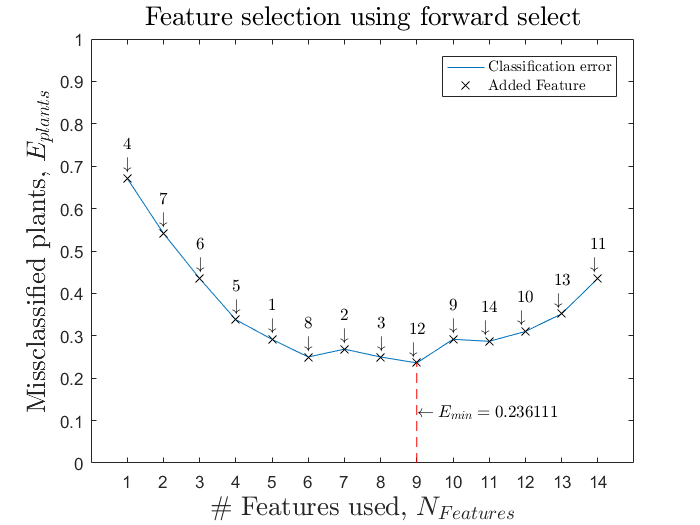
\includegraphics[width=\textwidth]{./figure/result/Quadratic/forward.png}
    \end{subfigure}
    \begin{subfigure}[b]{0.47\textwidth}
        \centering
        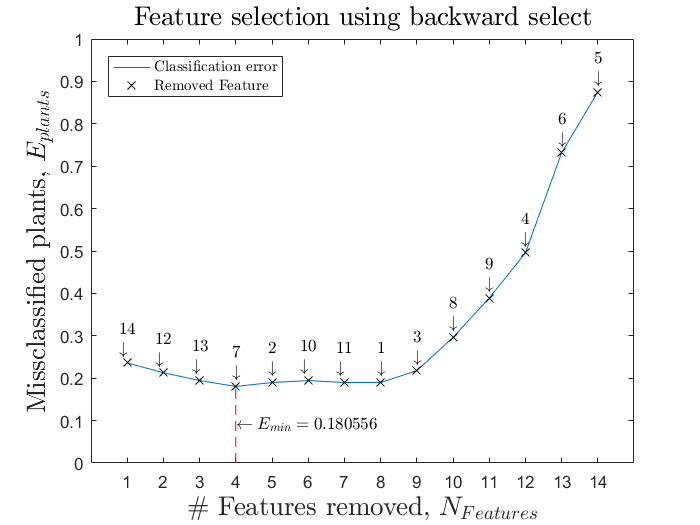
\includegraphics[width=\textwidth]{./figure/result/Quadratic/backward.png}
    \end{subfigure}
    \caption{\label{fig:backforSelection} Using either forward or backward selection for the best feature combination yields different results. E.g. Feature number 7 (mean blue) is the second feature to be added in the forward selection algorithm and is the last to be removed in the backward selection. The corresponding features can be found in Table~\ref{tab:featNameNum}.}
\end{figure}

\begin{figure}[H]
\centering
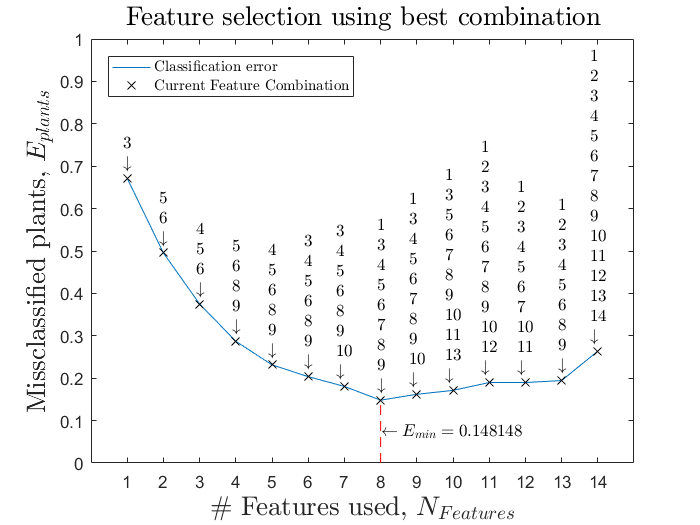
\includegraphics[width=0.47\textwidth]{./figure/result/Quadratic/combination.png}
\caption{\label{fig:combSelection} With immense computer power the best $n$ combinations can be found using brute force. This ensures to get the best available combination using $n$ features as all combinations are compared to each other.  }
\end{figure}

As we can see in Figure~\ref{fig:backforSelection}, many of the defined features are present when selecting the best combinations of features using both the backward and forward selection algorithm. In both cases, the class of features which are neglected the most are the moment invariant features. During these algorithms $K-$cross validation was used with $K=3$, i.e. the different plants was randomly divided into 9 different groups with 3 plants in each. This grouping is different for each run and might thus yield different results for different runs. To make this more consistent, the grouping could be done using the increasing dart wheel indexing as in Figure~\ref{fig:dartWheel} instead of the random distribution in Figure~\ref{fig:randomWheel}, but then we do not introduce the same amount of stochasticity in the training and is more prone to overfitting.

With much patient, the absolute best combination was found by combining the best $n$ features together. This can be seen in Figure~\ref{fig:combSelection}. The result from using this algorithm will only be used in a best case scenario when comparing to other methods later as this algorithm is very slow compared to the other. The feature selection process usually takes place before the classification is done, though, if one would find a new feature that might give more information this whole process would need to be made again and thus a fast algorithm is preferred.

\subsubsection{Feed forward neural network}

The neural network differs from the Quadratic Discriminant in several regards. Firstly, the model is not uniquely determined by the training instances, as each training data only updates the parameters of the model and not creates them, and also that the model can start overfitting due too to large exposure of the training data.\\



\begin{table}[]
\centering
\caption{The different feature selection models used in the Quadratic Discriminant model produces different combinations of features. These combination of features will be used as input to the neural networks. The numbers corresponds to the features in Table.~\ref{tab:featNameNum}.}
\label{fig:feat_select}
\begin{tabular}{|l|l|l|l|}
\hline
                         & Forward selection  & Backward Selection    & Best Combination   \\ \hline
\begin{tabular}[c]{@{}c@{}}Selected Feature\\ numbers\end{tabular} & 1 2 3 4 5 6 7 8 12 & 1 2 3 4 5 6 8 9 10 11 & 1 3 4 5 6 7 8 9 10 \\ \hline
\begin{tabular}[c]{@{}c@{}}Misclassified\\ plants\end{tabular} & 0.236 & 0.181 & 0.148 \\ \hline

\end{tabular}
\end{table}

The training of the networks takes more time than the Quadratic Discriminant and the feature selection process would therefore take much longer time for this approach. We will instead use the results from the previous model and apply the different feature combinations to this algorithm, meaning we will train 3 different networks, using the features from the, forward selection, backward selection, and best combination, as input to the networks. The combination of features gained from the previous model can be seen in Figure.~\ref{fig:feat_select}. The algorithm has been trained on the same division of the data and has been trained on different sized networks, both in the number of layers and the number of neurons in each layer. The networks has been trained for $10000$ epochs when 1 hidden layer is present and $100000$ with 2 hidden layers. The learning rate was set to $\alpha=0.01$ for all training instances. The data sets was divided in the same manner as for the Quadratic Discriminant, and thus 9 different networks are trained for each networks size, where the results of each network has been averaged. To find the best sized network for each combination of features we test different combinations until we find the best one. In Section~.\ref{sec:ffnn} we talked about that using a 2 hidden layered neural network is sufficient to separate data using arbitrary decision boundaries, which is also the limit of the network size tried. Deeper networks might be used for finding more complex patterns, but since we have well defined features we will not consider that approach. The different sizes for the networks that we will consider can be found in Table.~\ref{tab:nn_sizes}.

\begin{table}[]
\centering
\caption{Limiting the amount of nodes in each layer makes the training go faster than trying larger sizes and makes it easier to make exhaustive parameter space searches. A 2 hidden layer network with 5-15 nodes in each is considered, but also a 1 hidden layer network with 5-25 nodes.}
\label{tab:nn_sizes}
\begin{tabular}{|c|c|c|}
\hline
\multicolumn{1}{|l|}{}                                                    & \multicolumn{1}{l|}{Using 1 hidden layer} & \multicolumn{1}{l|}{Using 2 hidden layers} \\ \hline
\begin{tabular}[c]{@{}c@{}}\#Nodes\\ first hidden \\ layer\end{tabular}   & 5-25                                      & 5-15                                       \\ \hline
\begin{tabular}[c]{@{}c@{}}\#Nodes\\  second hidden \\ layer\end{tabular} & $\sim$                                    & 5-15                                       \\ \hline
\end{tabular}
\end{table}

The results from the different network sizes and different selected features can be seen in Table.~\ref{tab:nnres}.

\begin{table}[h]
    \centering
    \caption{Using different kinds of combinations of features give rise to differently clustered data. A neural network can separate data differently depending on the network sizes. Here is noted the best neural networks sizes for the three different results from the Quadratic Discriminant feature selection method. Both 1 hidden and 2 hidden layers are considered.}
    \label{tab:nnres}
    \begin{tabular}{|l|c|l|c|l|}
    \hline
    \begin{tabular}[c]{@{}l@{}}Feature Selection\\ From Quadratic\\ Discriminant\end{tabular} & \begin{tabular}[c]{@{}l@{}}1 Hidden \\ Layer\\ (Best Size)\end{tabular} & \begin{tabular}[c]{@{}l@{}}Misclassified \\ Plants\end{tabular} & \begin{tabular}[c]{@{}l@{}}2 Hidden \\ Layers\\ (Best Sizes)\end{tabular} & \begin{tabular}[c]{@{}l@{}}Misclassified \\ Plants\end{tabular} \\\hline
    Forward Selection
    & 16 & 0.148 & 8,8 & 0.153 \\\hline
    Backward Selection
    & 17 & 0.162 & 8,7 & 0.194\\\hline
    Best Combination
    & 20 & 0.125 & 13,7 & 0.176\\\hline
    \end{tabular}
\end{table}

\section{Data set 2}

The intended goal of the classification of the other data set is different from the first one, and thus it will be getting results from other algorithms.

\subsection{K-means Clustering}

The image segmentation method for this data set will not try to extract the objects from the background. Instead we will divide the image into $K$ different groups by applying the k-Means clustering algorithm on the pixel data. The pixels are transformed into several indices which are:

\begin{itemize}
    \item Red
    \item Green
    \item Blue
    \item Hue
    \item Saturation
    \item Intensity
    \item nDVi, green base
    \item nDVi, blue base
    \item Savi, green base
    \item Savi, blue base
    \item Masvi, green base
    \item Msavi, blue base
    \item Msavi2, green base
    \item Msavi2, blue base
\end{itemize}

To view the results of the clustering algorithm, each group is assigned a unique color, which makes it easy to see what part of the images that are assigned to each group. The result of this can be seen in Figure.~\ref{fig:kmeans}.

\begin{figure}[H]
    \centering
    \captionsetup[subfigure]{justification=centering}
    \begin{subfigure}[b]{0.49\textwidth}
        \centering
        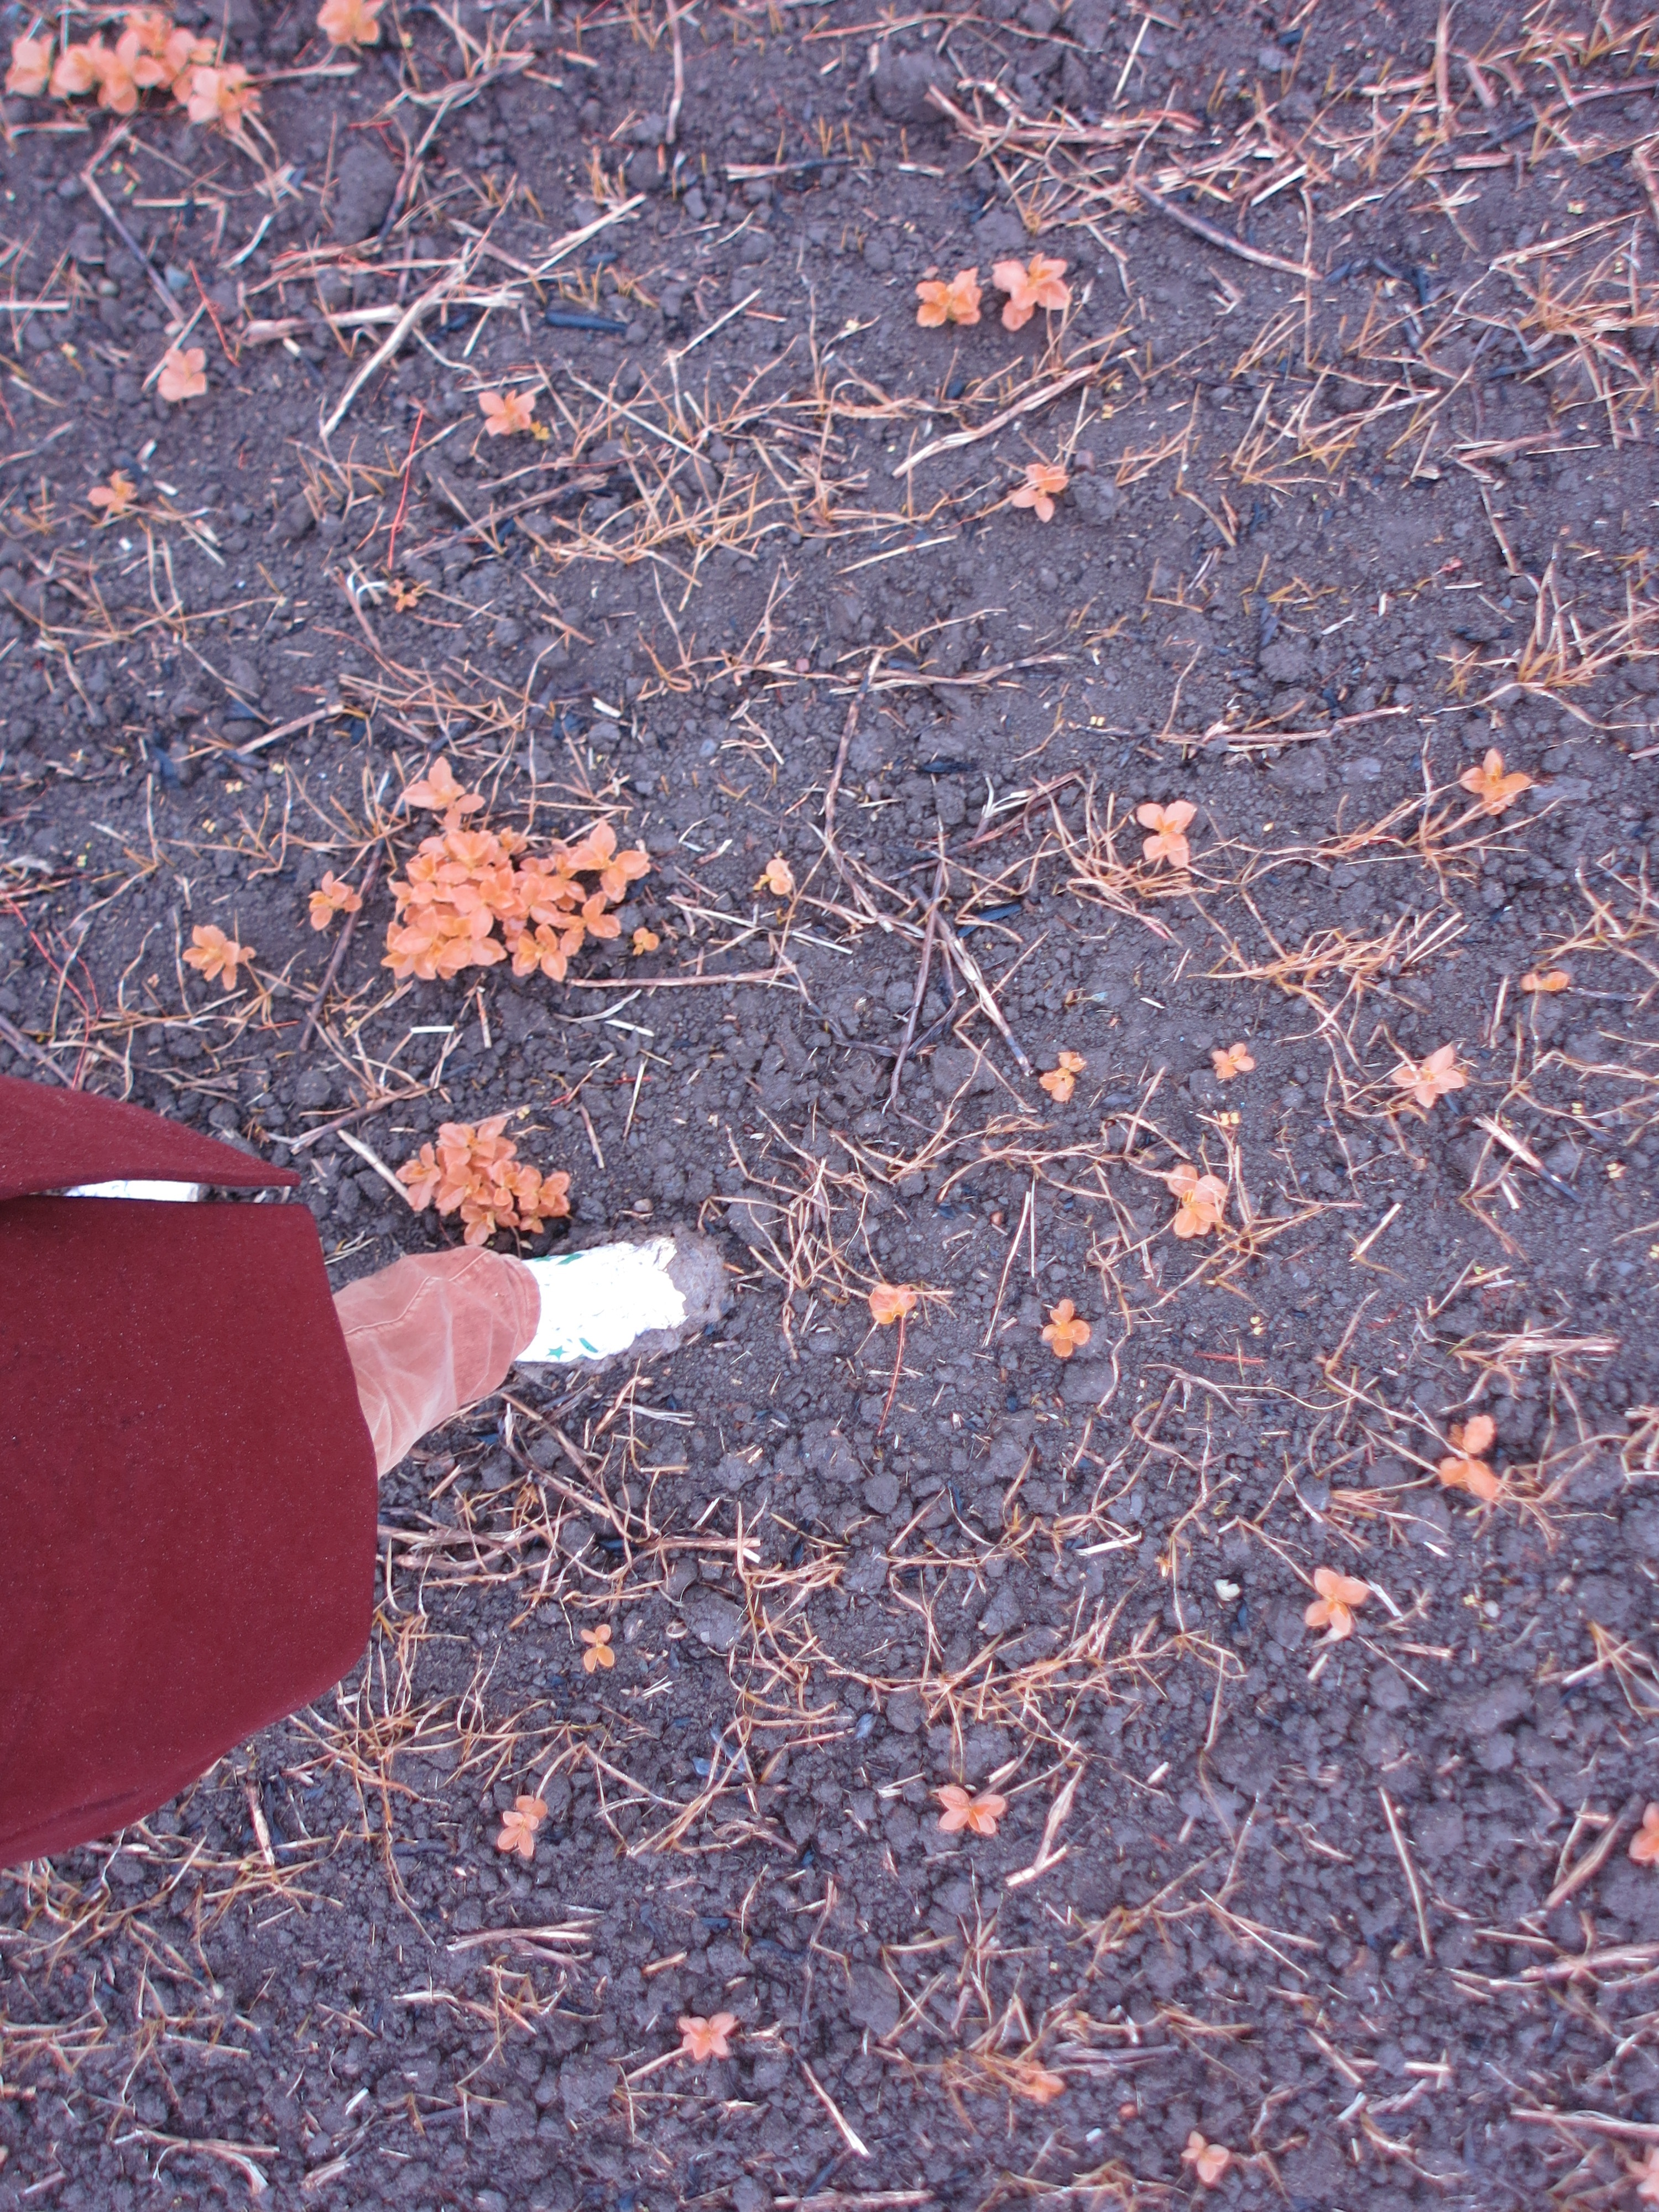
\includegraphics[width=\textwidth]{./figure/result/images/img_orig.jpg}
		\caption{}
		\label{fig:seg_a}
    \end{subfigure}
    \begin{subfigure}[b]{0.49\textwidth}
        \centering
        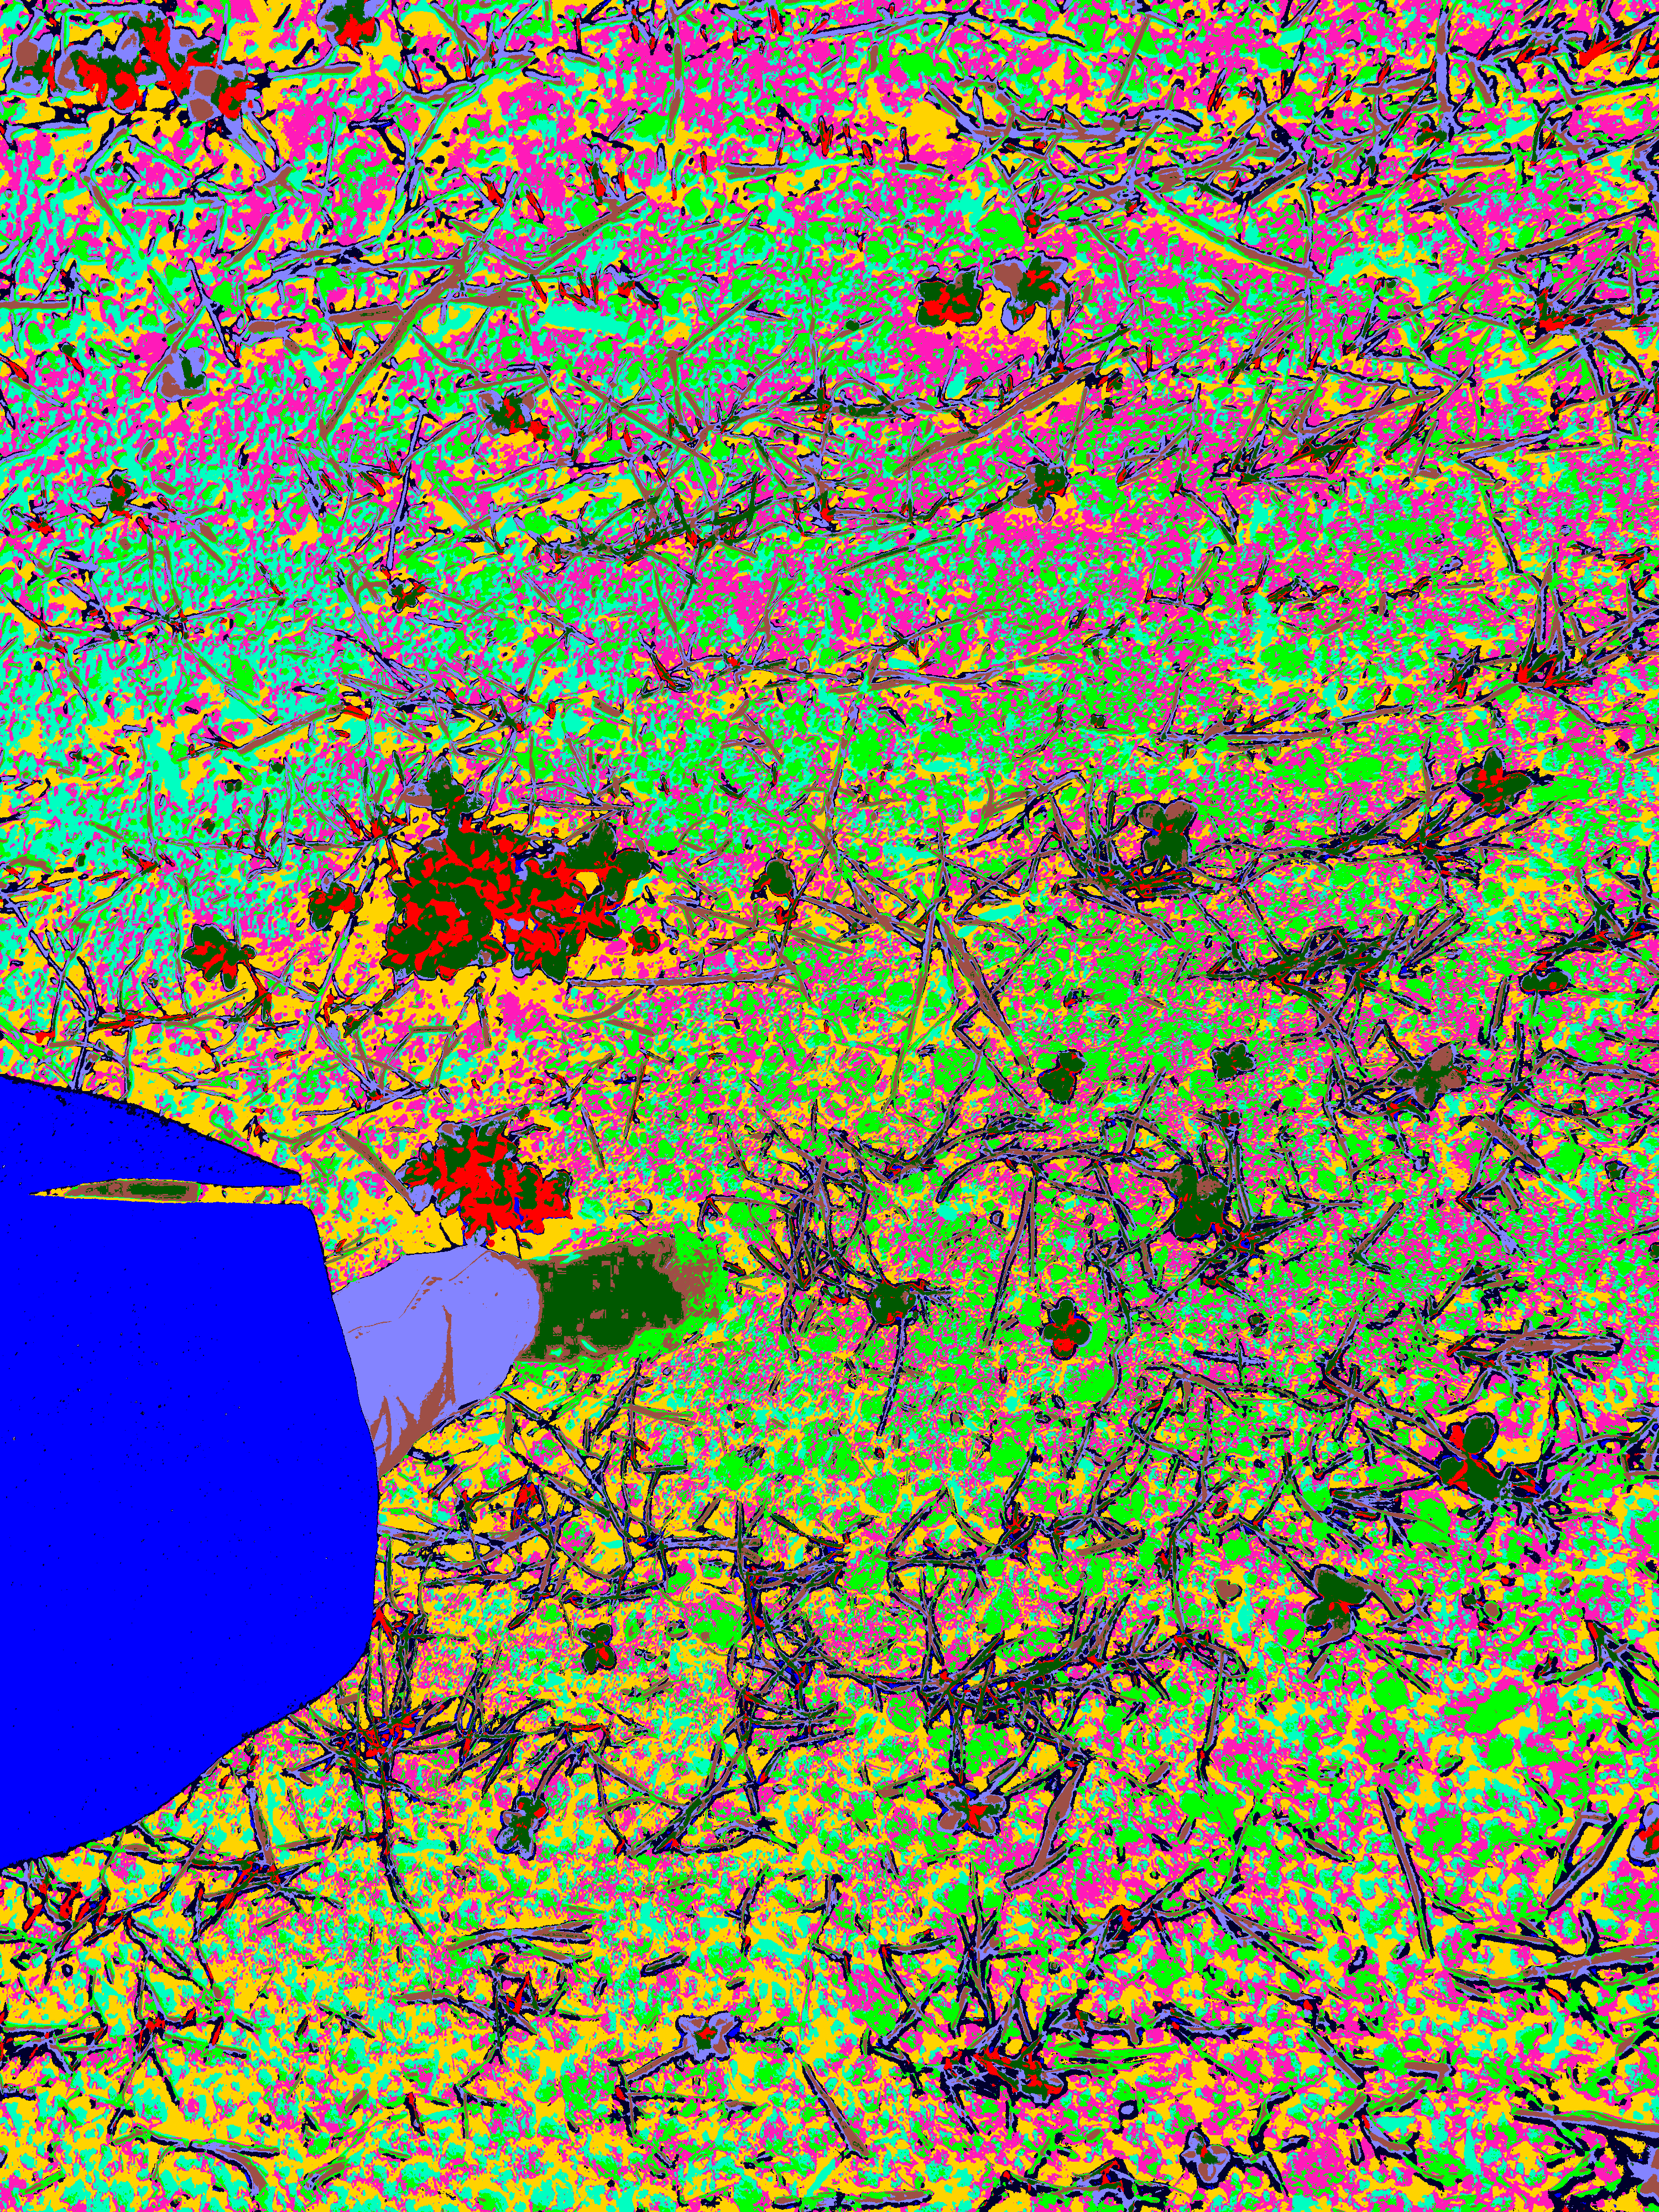
\includegraphics[width=\textwidth]{./figure/result/images/img_kmeans.png}
        \caption{}
		\label{fig:seg_b}
    \end{subfigure}
    \caption{The k-means clustering algorithm can create really interesting images by giving each pixel from the groups a common color. The algorithm seems to divide the image in several parts, where the background and the different kinds of plants are in different groups.}
    \label{fig:kmeans}
\end{figure}

\subsection{Algorithm evaluation}

This data set is harder to evaluate as there is no label for each pixel of each image. Instead, $400$ points has been randomized on the images, labelled by hand, either as background, crop, or weed. The $K$ different groups are then assigned the same label as the highest ranking label for that group according to Section.\ref{sec:unsupervised_method}.

5 images, meaning 2000 data points, was used as training, both for the k-means in the previous section and for the group classification. The evaluation of the algorithms is done by comparing the percentage of the points belonging to either a crop plant or a weed plant based on the classification by hand, with the same points after the training and classification. In Figure.~\ref{fig:k_means_grouping_result} we can see the results for both the training images and the test images. We can see a clear correlation between the ground truth percentages and the estimated percentages for both classes, and the calculated correlation coefficients can be seen in Table.~\ref{tab:corrcoef}. In both instances the estimated percentage seems to be underestimated, but it seems like this underestimation is rather consistent.

\begin{figure}[H]
    \centering
    \captionsetup[subfigure]{justification=centering}
    \begin{subfigure}[b]{0.49\textwidth}
        \centering
        % This file was created by matlab2tikz.
%
%The latest updates can be retrieved from
%  http://www.mathworks.com/matlabcentral/fileexchange/22022-matlab2tikz-matlab2tikz
%where you can also make suggestions and rate matlab2tikz.
%
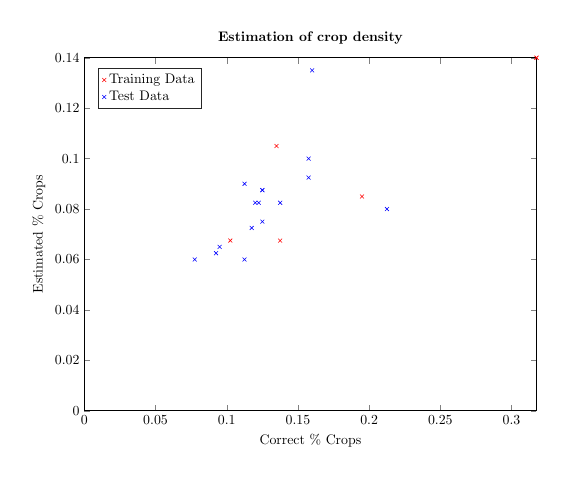
\begin{tikzpicture}[scale=0.5]

\begin{axis}[%
width=4.521in,
height=3.53in,
at={(0.758in,0.517in)},
scale only axis,
xmin=0,
xmax=0.3175,
xlabel={Correct $\%$ Crops},
ymin=0,
ymax=0.14,
ylabel={Estimated $\%$ Crops},
x tick label style={/pgf/number format/fixed},
y tick label style={/pgf/number format/fixed},
axis background/.style={fill=white},
title style={font=\bfseries},
title={Estimation of crop density},
legend style={at={(0.03,0.97)},anchor=north west,legend cell align=left,align=left,draw=white!15!black}
]
\addplot [color=red,only marks,mark=x,mark options={solid}]
  table[row sep=crcr]{%
0.3175	0.14\\
};
\addlegendentry{Training Data};

\addplot [color=blue,only marks,mark=x,mark options={solid}]
  table[row sep=crcr]{%
0.125	0.0875\\
};
\addlegendentry{Test Data};

\addplot [color=red,only marks,mark=x,mark options={solid},forget plot]
  table[row sep=crcr]{%
0.3175	0.14\\
};
\addplot [color=red,only marks,mark=x,mark options={solid},forget plot]
  table[row sep=crcr]{%
0.195	0.085\\
};
\addplot [color=red,only marks,mark=x,mark options={solid},forget plot]
  table[row sep=crcr]{%
0.1025	0.0675\\
};
\addplot [color=red,only marks,mark=x,mark options={solid},forget plot]
  table[row sep=crcr]{%
0.1375	0.0675\\
};
\addplot [color=red,only marks,mark=x,mark options={solid},forget plot]
  table[row sep=crcr]{%
0.135	0.105\\
};
\addplot [color=blue,only marks,mark=x,mark options={solid},forget plot]
  table[row sep=crcr]{%
0.125	0.0875\\
};
\addplot [color=blue,only marks,mark=x,mark options={solid},forget plot]
  table[row sep=crcr]{%
0.1575	0.0925\\
};
\addplot [color=blue,only marks,mark=x,mark options={solid},forget plot]
  table[row sep=crcr]{%
0.2125	0.08\\
};
\addplot [color=blue,only marks,mark=x,mark options={solid},forget plot]
  table[row sep=crcr]{%
0.1575	0.1\\
};
\addplot [color=blue,only marks,mark=x,mark options={solid},forget plot]
  table[row sep=crcr]{%
0.125	0.075\\
};
\addplot [color=blue,only marks,mark=x,mark options={solid},forget plot]
  table[row sep=crcr]{%
0.095	0.065\\
};
\addplot [color=blue,only marks,mark=x,mark options={solid},forget plot]
  table[row sep=crcr]{%
0.1125	0.09\\
};
\addplot [color=blue,only marks,mark=x,mark options={solid},forget plot]
  table[row sep=crcr]{%
0.1225	0.0825\\
};
\addplot [color=blue,only marks,mark=x,mark options={solid},forget plot]
  table[row sep=crcr]{%
0.12	0.0825\\
};
\addplot [color=blue,only marks,mark=x,mark options={solid},forget plot]
  table[row sep=crcr]{%
0.1375	0.0825\\
};
\addplot [color=blue,only marks,mark=x,mark options={solid},forget plot]
  table[row sep=crcr]{%
0.1125	0.06\\
};
\addplot [color=blue,only marks,mark=x,mark options={solid},forget plot]
  table[row sep=crcr]{%
0.16	0.135\\
};
\addplot [color=blue,only marks,mark=x,mark options={solid},forget plot]
  table[row sep=crcr]{%
0.1175	0.0725\\
};
\addplot [color=blue,only marks,mark=x,mark options={solid},forget plot]
  table[row sep=crcr]{%
0.0925	0.0625\\
};
\addplot [color=blue,only marks,mark=x,mark options={solid},forget plot]
  table[row sep=crcr]{%
0.0775	0.06\\
};
\end{axis}
\end{tikzpicture}%

    \end{subfigure}
    \begin{subfigure}[b]{0.49\textwidth}
        \centering
        % This file was created by matlab2tikz.
%
%The latest updates can be retrieved from
%  http://www.mathworks.com/matlabcentral/fileexchange/22022-matlab2tikz-matlab2tikz
%where you can also make suggestions and rate matlab2tikz.
%
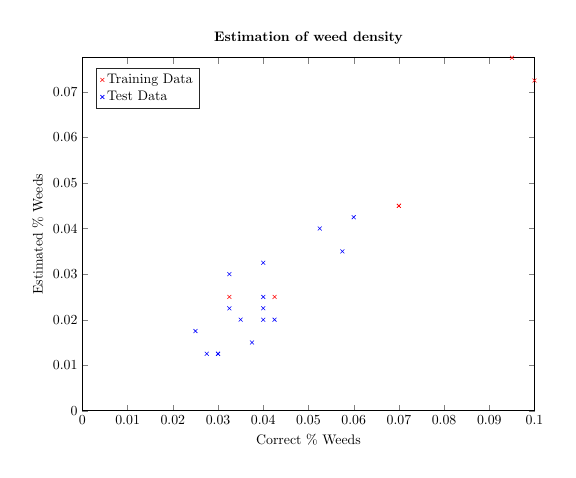
\begin{tikzpicture}[scale=0.5]

\begin{axis}[%
width=4.521in,
height=3.53in,
at={(0.758in,0.517in)},
scale only axis,
xmin=0,
xmax=0.1,
xlabel={Correct $\%$ Weeds},
ymin=0,
ymax=0.0775,
ylabel={Estimated $\%$ Weeds},
tick label style={/pgf/number format/fixed},
scaled y ticks=false,
axis background/.style={fill=white},
title style={font=\bfseries},
title={Estimation of weed density},
legend style={at={(0.03,0.97)},anchor=north west,legend cell align=left,align=left,draw=white!15!black}
]
\addplot [color=red,only marks,mark=x,mark options={solid}]
  table[row sep=crcr]{%
0.07	0.045\\
};
\addlegendentry{Training Data};

\addplot [color=blue,only marks,mark=x,mark options={solid}]
  table[row sep=crcr]{%
0.03	0.0125\\
};
\addlegendentry{Test Data};

\addplot [color=red,only marks,mark=x,mark options={solid},forget plot]
  table[row sep=crcr]{%
0.07	0.045\\
};
\addplot [color=red,only marks,mark=x,mark options={solid},forget plot]
  table[row sep=crcr]{%
0.1	0.0725\\
};
\addplot [color=red,only marks,mark=x,mark options={solid},forget plot]
  table[row sep=crcr]{%
0.095	0.0775\\
};
\addplot [color=red,only marks,mark=x,mark options={solid},forget plot]
  table[row sep=crcr]{%
0.0425	0.025\\
};
\addplot [color=red,only marks,mark=x,mark options={solid},forget plot]
  table[row sep=crcr]{%
0.0325	0.025\\
};
\addplot [color=blue,only marks,mark=x,mark options={solid},forget plot]
  table[row sep=crcr]{%
0.03	0.0125\\
};
\addplot [color=blue,only marks,mark=x,mark options={solid},forget plot]
  table[row sep=crcr]{%
0.025	0.0175\\
};
\addplot [color=blue,only marks,mark=x,mark options={solid},forget plot]
  table[row sep=crcr]{%
0.0425	0.02\\
};
\addplot [color=blue,only marks,mark=x,mark options={solid},forget plot]
  table[row sep=crcr]{%
0.0275	0.0125\\
};
\addplot [color=blue,only marks,mark=x,mark options={solid},forget plot]
  table[row sep=crcr]{%
0.04	0.025\\
};
\addplot [color=blue,only marks,mark=x,mark options={solid},forget plot]
  table[row sep=crcr]{%
0.0575	0.035\\
};
\addplot [color=blue,only marks,mark=x,mark options={solid},forget plot]
  table[row sep=crcr]{%
0.0325	0.0225\\
};
\addplot [color=blue,only marks,mark=x,mark options={solid},forget plot]
  table[row sep=crcr]{%
0.0375	0.015\\
};
\addplot [color=blue,only marks,mark=x,mark options={solid},forget plot]
  table[row sep=crcr]{%
0.04	0.02\\
};
\addplot [color=blue,only marks,mark=x,mark options={solid},forget plot]
  table[row sep=crcr]{%
0.035	0.02\\
};
\addplot [color=blue,only marks,mark=x,mark options={solid},forget plot]
  table[row sep=crcr]{%
0.06	0.0425\\
};
\addplot [color=blue,only marks,mark=x,mark options={solid},forget plot]
  table[row sep=crcr]{%
0.04	0.0225\\
};
\addplot [color=blue,only marks,mark=x,mark options={solid},forget plot]
  table[row sep=crcr]{%
0.0325	0.03\\
};
\addplot [color=blue,only marks,mark=x,mark options={solid},forget plot]
  table[row sep=crcr]{%
0.04	0.0325\\
};
\addplot [color=blue,only marks,mark=x,mark options={solid},forget plot]
  table[row sep=crcr]{%
0.0525	0.04\\
};
\end{axis}
\end{tikzpicture}%

    \end{subfigure}
    \caption{The figures show the result for after the labelling of the clusters in the k-means algorithm. In the left we can see the ground truths percentage plotted against the estimation in the algorithm for the crops and the same but for the weeds in the right. The red crosses denoted the training instances and the blue ones are the test images. A clear correlation between the axis data can be seen.}
    \label{fig:k_means_grouping_result}
\end{figure}


\begin{table}[]
\centering
\caption{The calculated correlation coefficients for between the ground truth and the estimated for crop and weeds estimations are close to the maximum value of 1.}
\label{tab:corrcoef}
\begin{tabular}{|l|l|}
\hline
      & \begin{tabular}[c]{@{}l@{}}Correlation \\ coefficient, $\rho$\end{tabular} \\ \hline
Weed & 0.8                                                             \\ \hline
Crop  & 0.55                                                                 \\ \hline
\end{tabular}
\end{table}

When we sort an entire image into the three groups, background, crop, and weed, based on the k-means clustering on the whole image we can see that the algorithm creates a good estimate for where each class is located in the image. The result of this can be seen in Figure.~\ref{fig:visual_result}.

\begin{figure}[H]
    \centering
    \captionsetup[subfigure]{justification=centering}
    \begin{subfigure}[b]{0.49\textwidth}
        \centering
        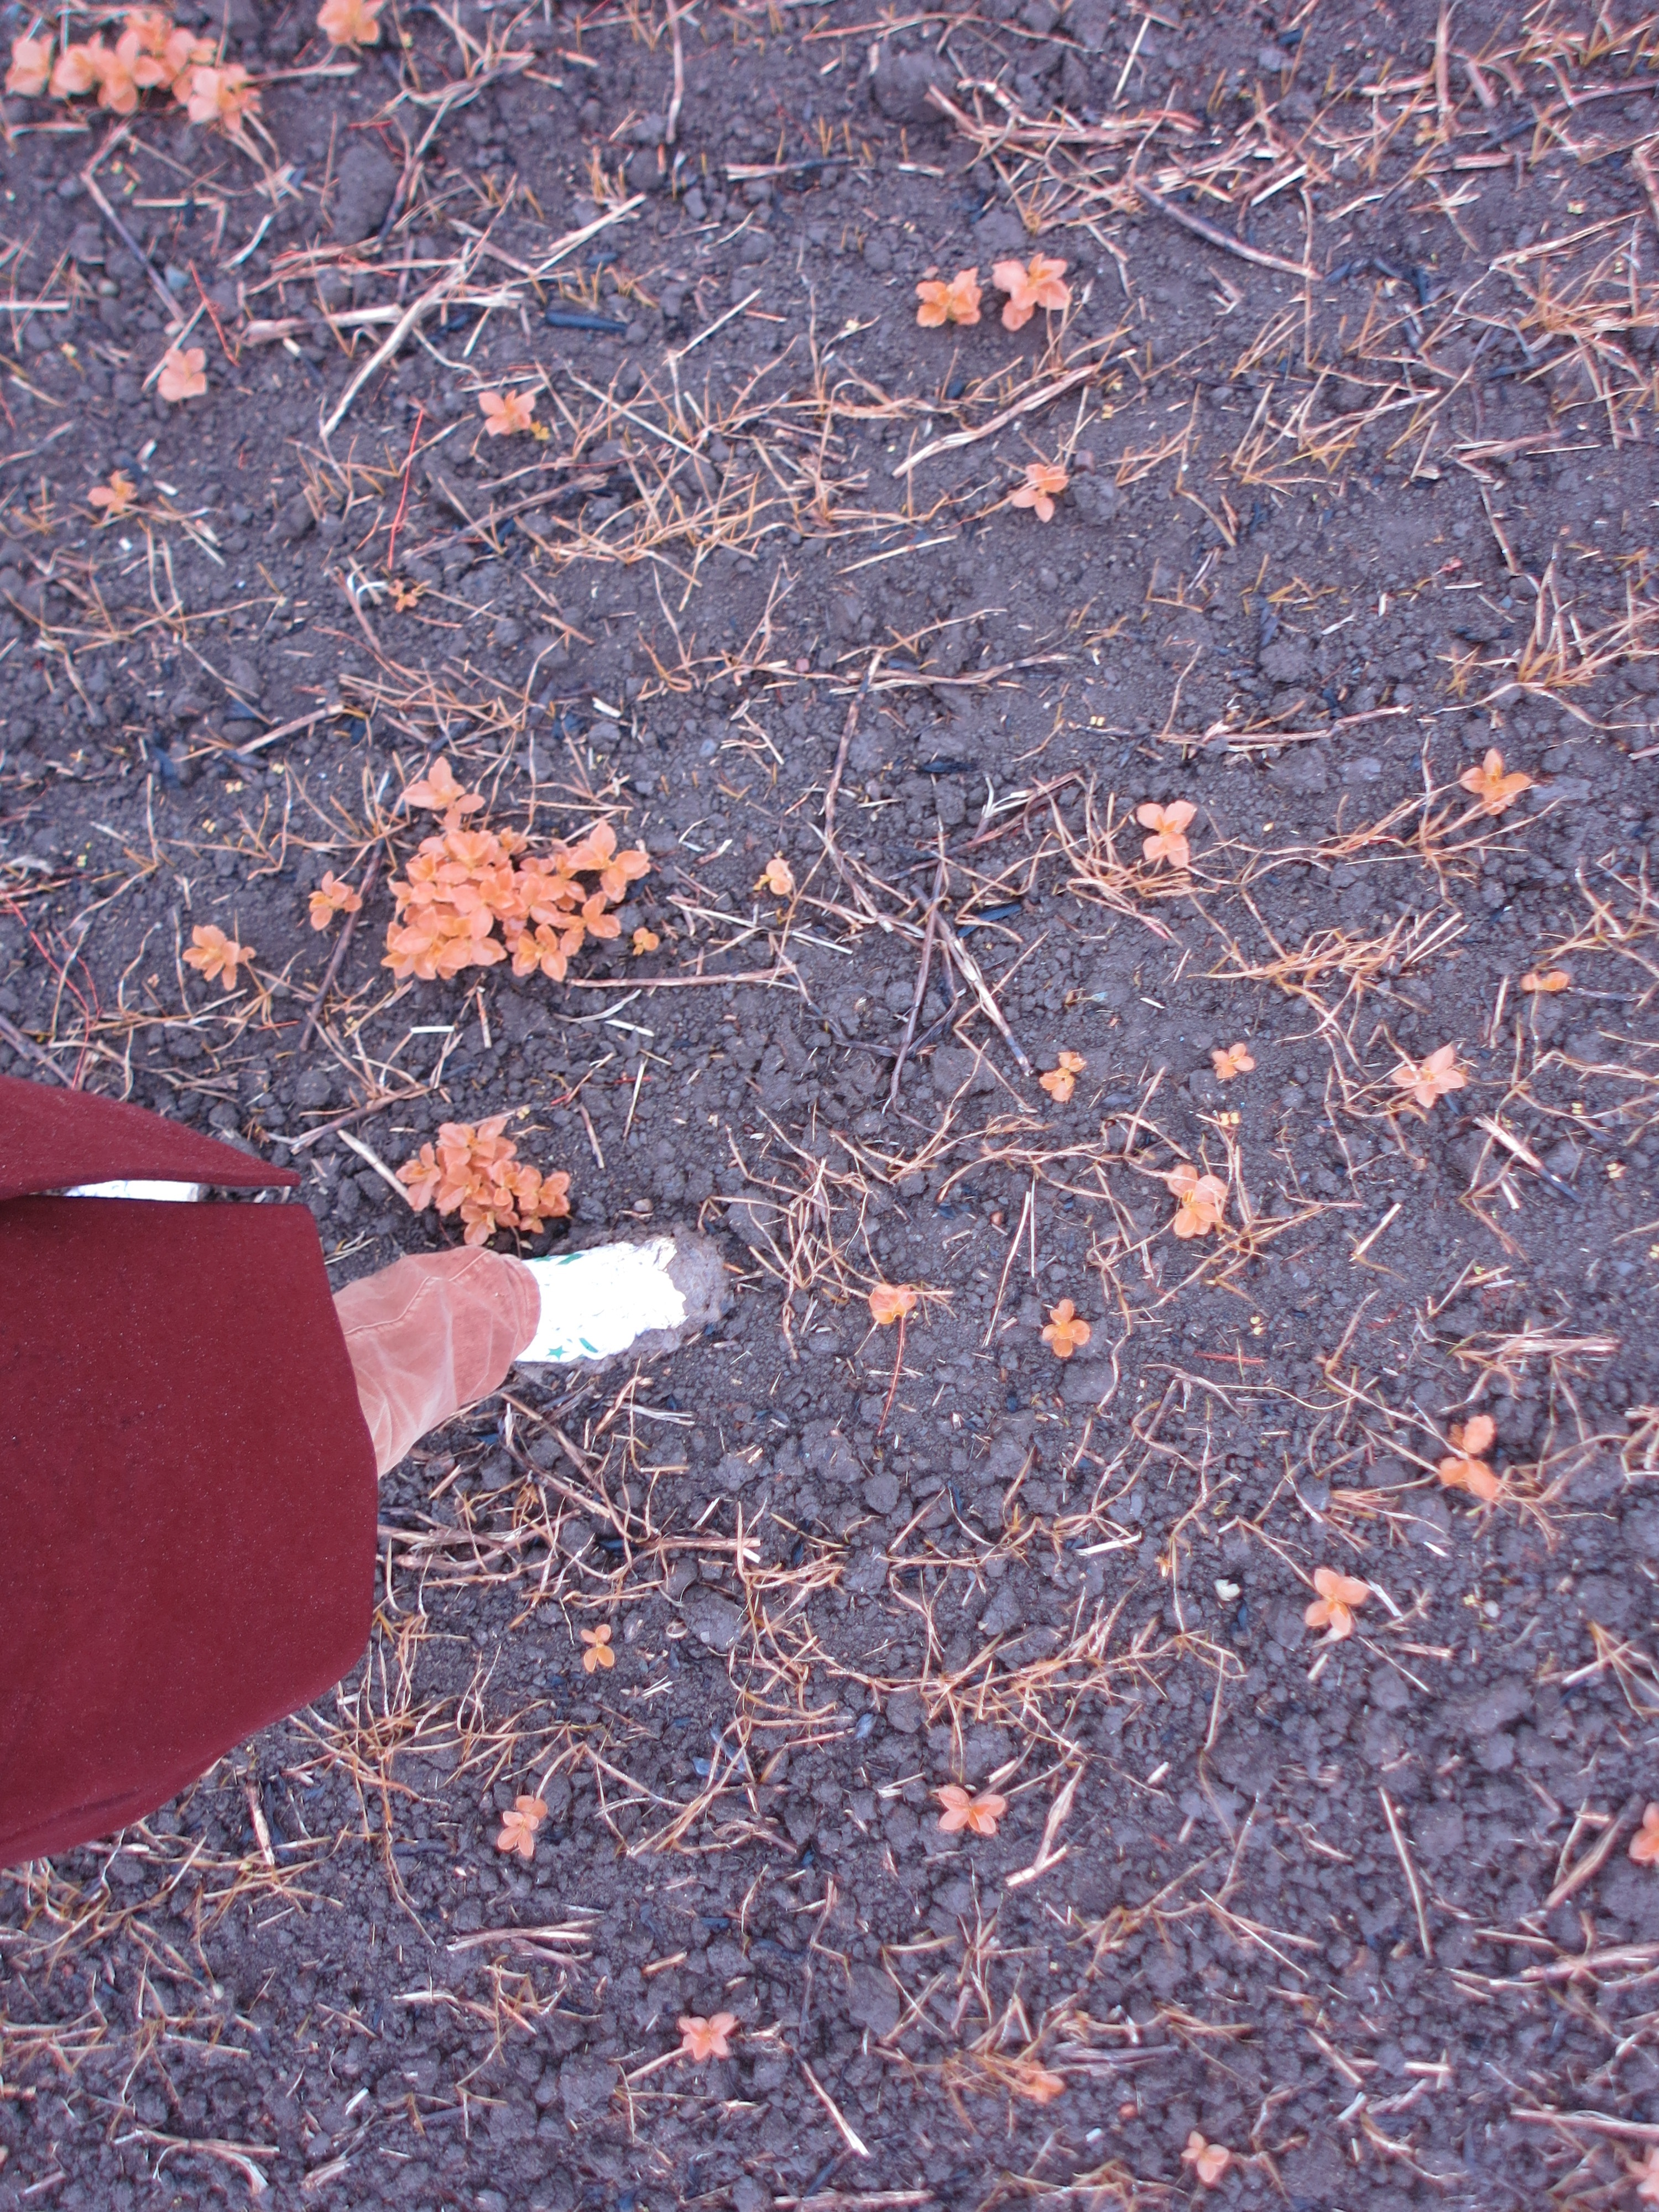
\includegraphics[width=\textwidth]{./figure/result/images/img_orig.jpg}
    \end{subfigure}
    \begin{subfigure}[b]{0.49\textwidth}
        \centering
        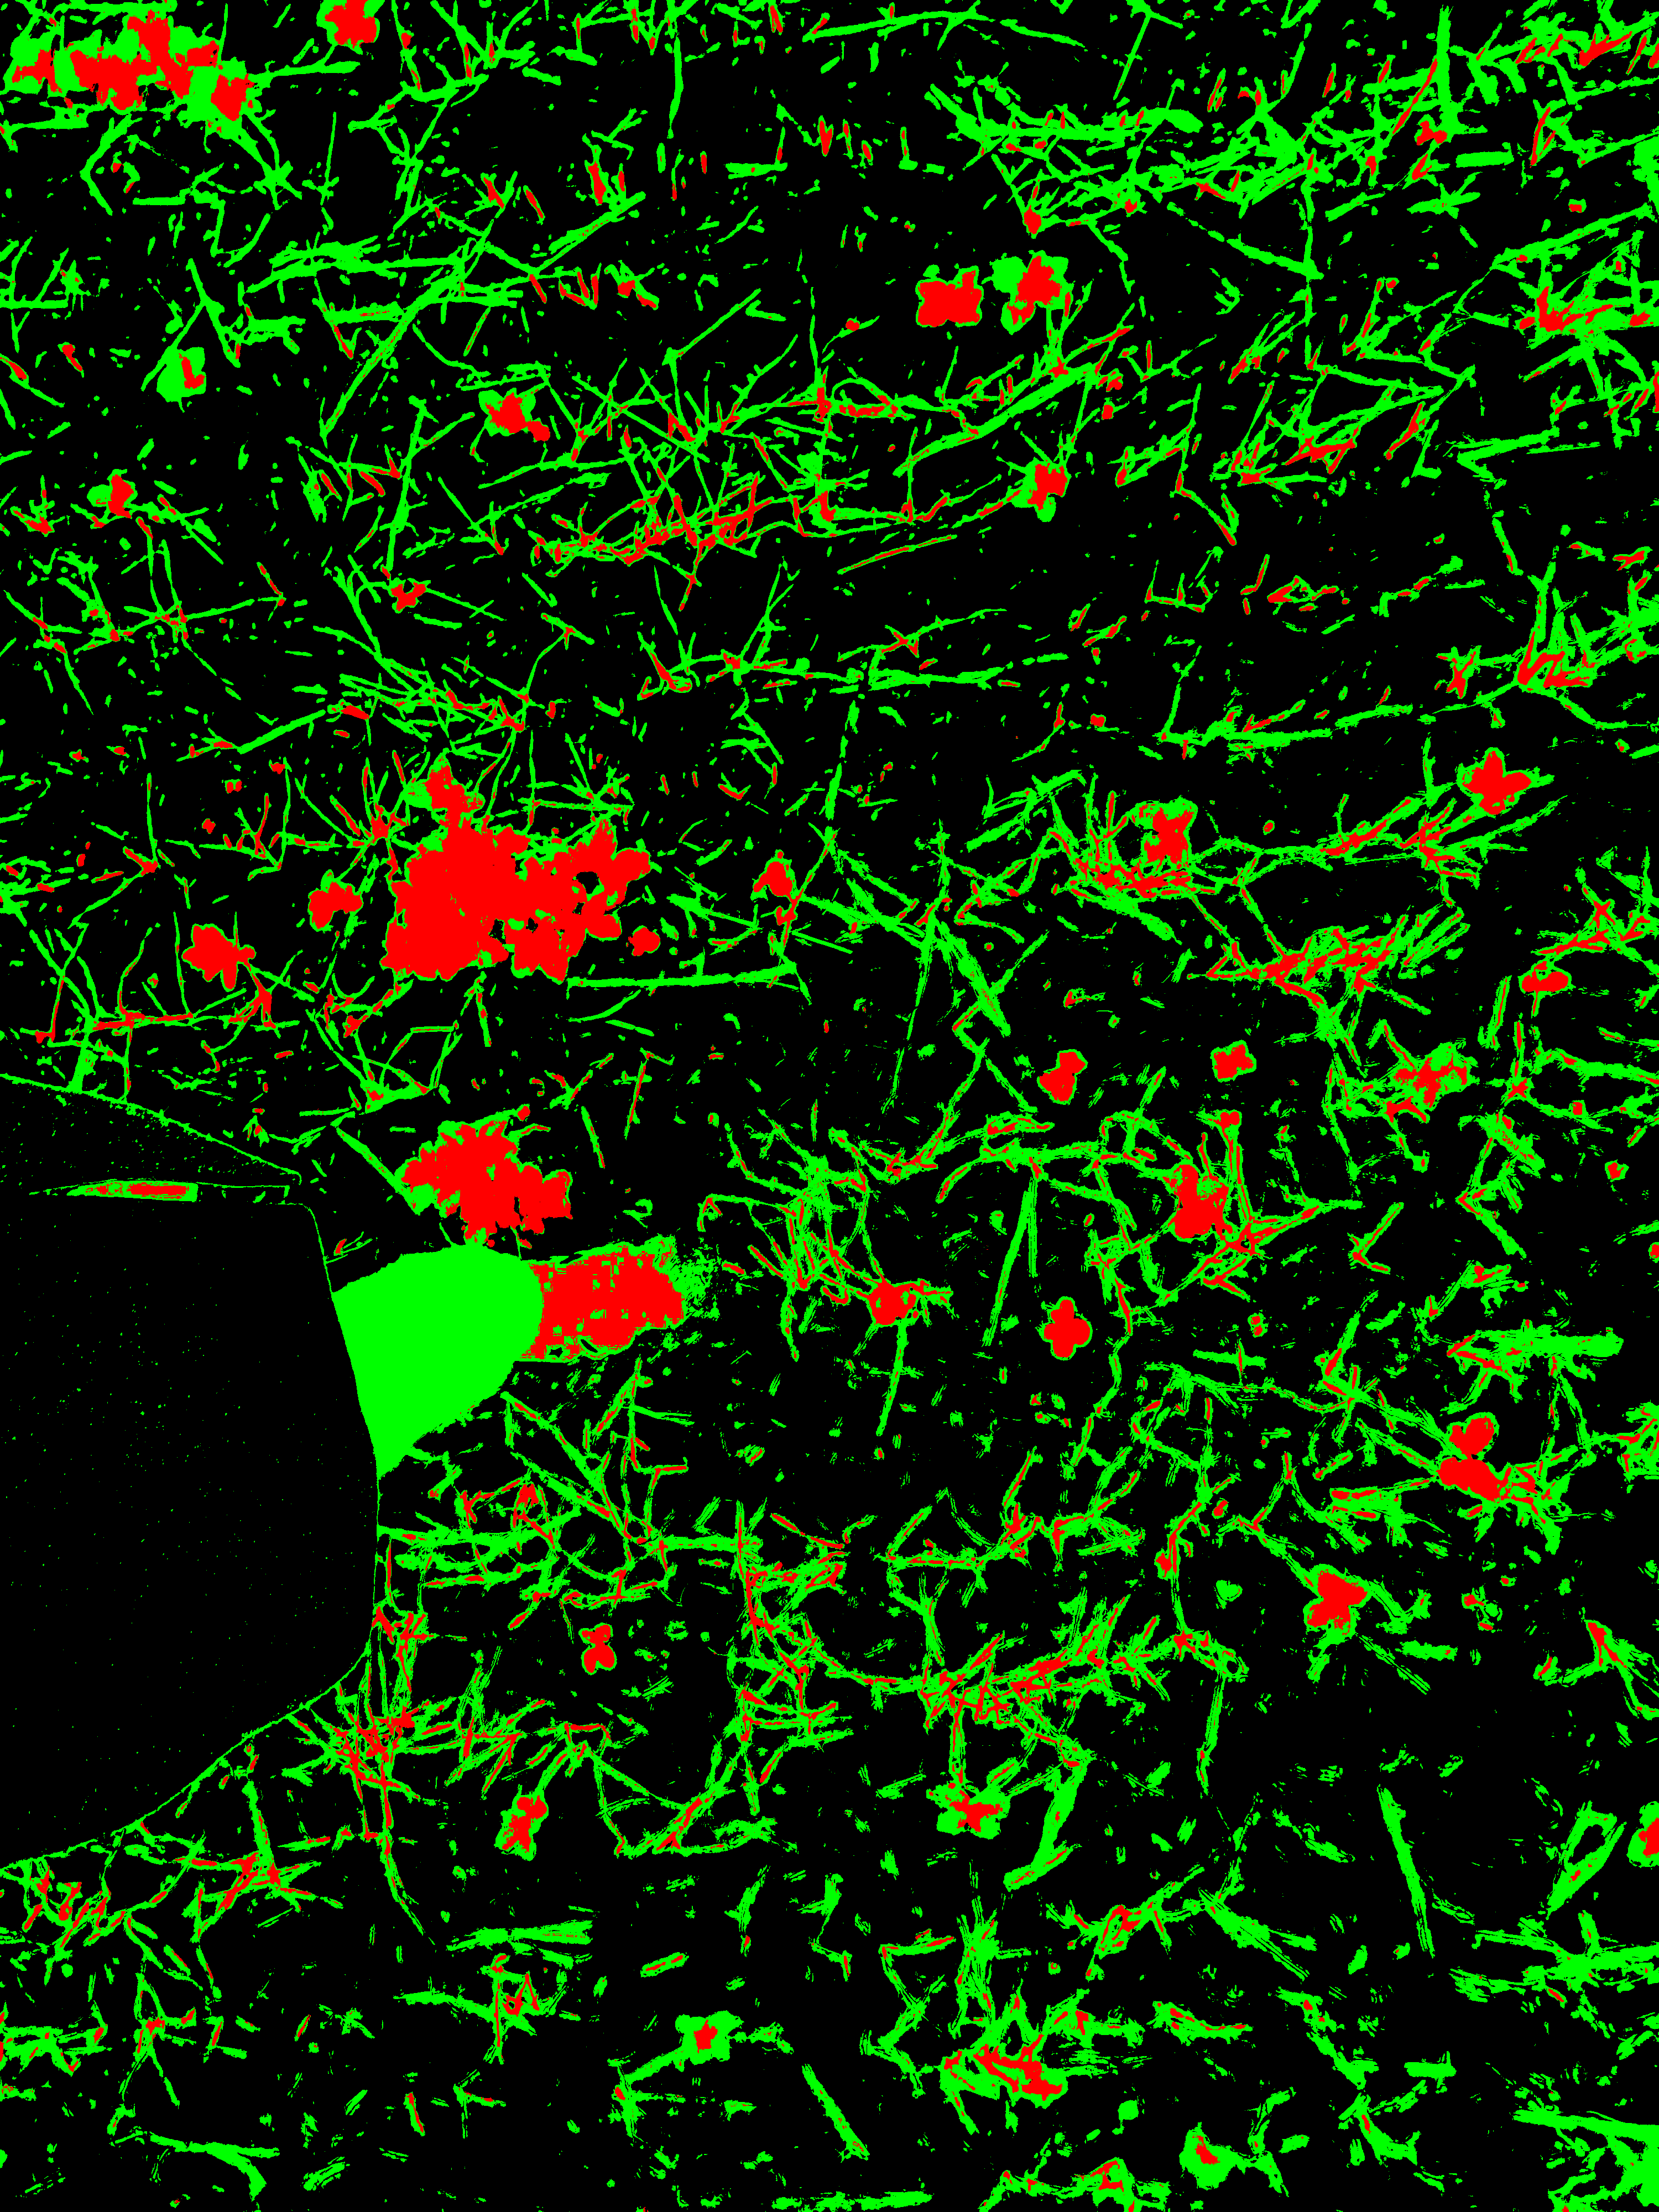
\includegraphics[width=\textwidth]{./figure/result/images/img_res.png}
    \end{subfigure}
    \caption{Applying the algorithm to an entire image produces quite appealing results. The green part on the image on the right is the estimated weed and the red are the estimated crops. There are large areas which seems to be correct, but there are some that should be labelled as the background. }
    \label{fig:visual_result}
\end{figure}
